\documentclass[12pt]{article}
\setlength{\oddsidemargin}{0in}
\setlength{\evensidemargin}{0in}
\setlength{\textwidth}{6.5in}
\setlength{\parindent}{0in}
\setlength{\parskip}{0.5 \baselineskip}
\usepackage[top = 1in, bottom = 1in]{geometry}

\usepackage[utf8]{inputenc}
\usepackage{amsmath,amsfonts,amssymb,mathtools,hyperref,graphicx, subcaption, float}
\mathtoolsset{showonlyrefs}
\setcounter{MaxMatrixCols}{20}

%\usepackage{titling}
%\setlength{\droptitle}{-1in}
\title{Using Linear Programming to Find Shortest Path}
\author{Darice Guittet and Benjamin Shoeman}
\date{8 November 2017}

\begin{document}

\maketitle

\section{Abstract}



\section{Introduction}
The problem of optimization arises in many contexts, from logistical considerations such as scheduling appointments, to financial concerns such as maximizing return from investments, to technical questions regarding control of interconnected systems, such as a power grid network. Linear programming is a group of techniques for tackling such problems when the system and its constraints can be represented linearly. Specifically, we investigate the Simplex Algorithm, which is a simple approach which can be proven via the Duality Theorem to return the optimal value, provided such a feasible solution exists. We apply our Simplex solver on the shortest-path problem on a graph by formulating it as a minimum flow problem. While the formulation can be generalized to more complex flow problems, we turn to the problem of finding the shortest path to reach one location on campus from another. When a student has only ten minutes between classes to get to another, an optimal path is desirable. 

\subsection{Linear Programs}
Linear programming is the process of optimizing a system by maximizing or minimizing an objective function given inequalities as constraints. Suppose we want to find the $n$ values of $x_1, x_2, \ldots, x_n \geq 0$ that maximize the objective function:

\begin{center}
     $c_1x_1 + \cdots + c_nx_n = \mathbf{c}^\text{T}\mathbf{x} = z(\mathbf{x})$\\
\end{center}

subject to the $m$ constraints:
\begin{center}
    $x_1a_{1,1} +  \cdots + x_ia_{1,i} + \cdots +  x_na_{1,n} \leq b_1$ \\
\hspace{0cm} \vdots \\
    $x_1a_{m,1} + \cdots + x_ia_{m,i} + \cdots +  x_ma_{m,n} \leq b_m$ \\
    $x_1, x_2, \cdots, x_n \geq 0$
\end{center} 

The coefficients vector of the objective function, $\mathbf{c} \in \mathbb{R}^n$, represents the cost or value of each element $x_i$, and the vector $\mathbf{b} \in \mathbb{R}^m$ represents requirements on properties of $x$, tabulated by the matrix $A_{m,n}$. By requiring nonnegativity of $x_i$ in the last constraint, we put the problem into standard form. All problems can be put into standard form \cite{ferguson}, in which all constraints are inequalities and $\mathbf{x}\geq0$, so the following theory regarding standard problems applies to general problems. The standard maximum problem can be written as:
\begin{equation} \label{eq:maxprob}
    \begin{array}{rrcl}
        \text{maximize} & z(\mathbf{x}) & = & \mathbf{c}^\text{T} \mathbf{x} \\
        \text{subject\ to} & A \mathbf{x} & \leq & \mathbf{b} \\
        \text{where} & \mathbf{x} & \geq & \mathbf{0}
    \end{array}
\end{equation}

Geometrically, each inequality cuts the space into half, where one side satisfies the inequality, and a collection of inequalities cuts the space into a polytope that defines the feasible region.

\begin{figure}[H]
\centering
    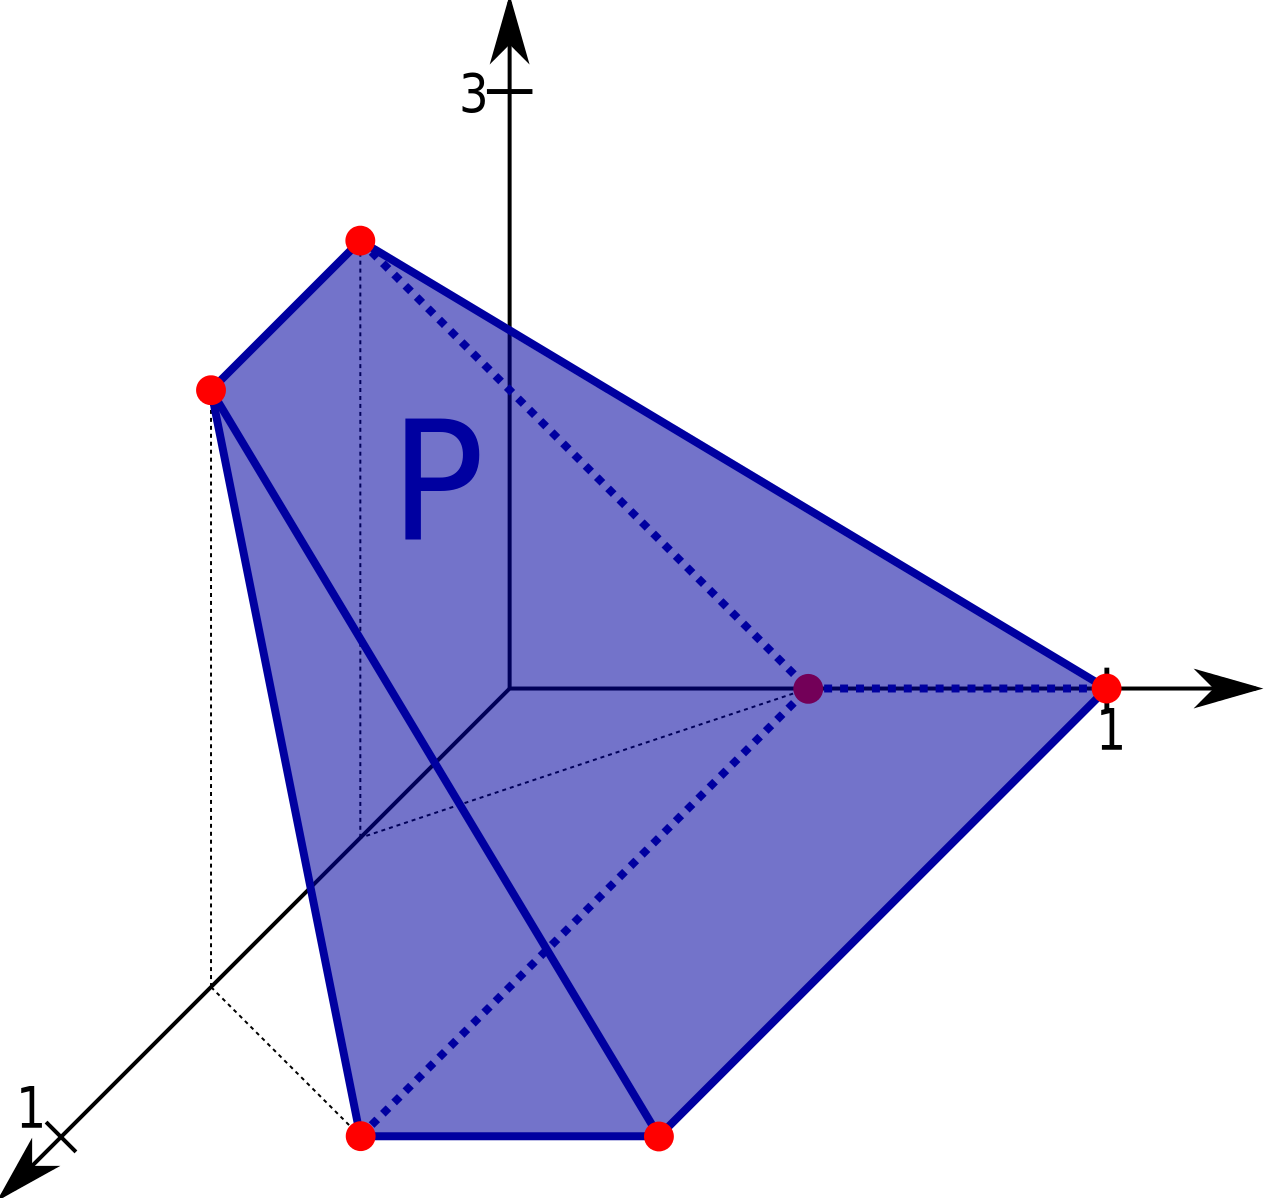
\includegraphics[width=2.5in]{3dpoly}
    \caption{Polyhedron in 3D Space. Picture from Wikipedia.}
\end{figure}

The objective function is also a line, and at each point, the objective function divides the space into a region with higher and lower values. So by traversing the edges towards higher values, the search space is reduced and eventually we find that the solution either lies on a vertex of the polytope or one of the edges is unbounded \cite{murty}. 

Not every optimization problem has an optimal solution, and if it exists, not every optimization technique is guaranteed to find it, especially if the dimension of the search space is very large and the relationships are non-linear. In our case for linear programs, the Simplex method can be proven to either find the optimal solution or show that it is infeasible, which makes it mathematically interesting, but the time it takes to do so is exponential in the size of the input, so it might be a poor choice for figuring out the best way to drive from Los Angeles to Boston (solution: drive on I-40 E for about 3,000 miles). 

\section{Mathematical Formulation}
\subsection{Does an Optimal Solution Exist?}
A linear program can be: feasible bounded, if a solution exists and the objective function is bounded; feasible unbounded, if a solution exists but the objective function can assume arbitrarily large values; or infeasible. We summarize the approaches in \cite{ferguson, trevisan} for showing that if an optimal solution exists, the Simplex method can find it.

The dual of the maximum problem \eqref{eq:maxprob} is the minimum problem. The maximum problem can be converted into its dual using the fact that $(a \leq b \land c \leq d) \implies y_1a+y_2c \leq y_1b+y_2d$, for some scaling factors $y_1, y_2 \in \mathbb{R}$. 

For each constraint in the maximum problem, we can derive a new inequality by scaling each and looking at the sum:

\begin{center}
    $y_1\big(x_1a_{1,1} +  \cdots + x_ia_{1,i} + \cdots +  x_na_{1,n}\big)$ + \\
    $\cdots$ \\
    $+ \ y_m\big( x_1a_{m,1} + \cdots + x_ia_{m,i} + \cdots +  x_ma_{m,n} \big) $\\
    $ \leq$ \\
    $ y_1b_1  + \cdots +  y_mb_m$ 
\end{center} 

We rewrite the inequality by gathering $x_i$ terms and find that for every feasible $\mathbf{x}$, a linear combination of the $x_i$ must be less than an upper bound $\mathbf{y}^\text{T}\mathbf{b}$.

\begin{center}
    $x_1 \big(y_1a_{1,1} +  \cdots + y_ia_{i,1} + \cdots +  y_ma_{m,1}\big)$ + \\
    $\cdots$ \\
    $+ \ x_n\big(y_1a_{1,n} + \cdots + y_ia_{i,n} + \cdots +  y_ma_{m,n} \big) $\\
    $ \leq$ \\
    $ y_1b_1  + \cdots +  y_mb_m$ 
\end{center} 

If we choose $y_i$ such that they satisfy the following constraints, where $c_i$ are the coefficients of the objective function,

\begin{center}
	$c_1 \leq y_1a_{1,1} +  \cdots + y_ia_{i,1} + \cdots +  y_ma_{m,1}$ \\
\hspace{0cm} \vdots \\
	$c_n \leq y_1a_{1,n} +  \cdots + y_ia_{i,n} + \cdots +  y_ma_{m,n}$ \\
\end{center}

and multiply the $i$ inequality by $x_i$ while summing each inequality as we did before, we arrive at a lower bound for the same linear combination of the $x_i$ for which we found an upper bound.

\begin{center}
	$ c_1x_1 + \cdots + c_nx_n  $ \\
	$ \leq $\\
    $x_1 \big(y_1a_{1,1} +  \cdots + y_ia_{i,1} + \cdots +  y_ma_{m,1}\big)$ + \\
    $\cdots$ \\
    $+ \ x_n\big(y_1a_{1,n} + \cdots + y_ia_{i,n} + \cdots +  y_ma_{m,n} \big) $\\
    $ \leq$ \\
    $ y_1b_1  + \cdots +  y_mb_m$ 
\end{center} 

The dual of the standard maximum problem \eqref{eq:maxprob}, the standard minimum problem, comes from solving for the scaling factors $y_i$ for which we get as tight of an upper bound as possible:

\begin{equation} \label{eq:minprob}
    \begin{array}{rrcl}
        \text{minimize} & z'(\mathbf{y}) & = & \mathbf{y}^\text{T} \mathbf{b} \\
        \text{subject\ to} & A^\text{T} \mathbf{y} & \geq & \mathbf{c} \\
        \text{where} & \mathbf{y} & \geq & \mathbf{0}
    \end{array}
\end{equation}
where $\mathbf{c} \in \mathbb{R}^n$, $\mathbf{y} \in \mathbb{R}^m$ and matrix $A^\text{T}$ is size $n$ x $m$.

In fact, the dual of the dual of the linear program is the linear program itself, called the \textit{primal} \cite{trevisan}, which can be formed by taking the negative of \eqref{eq:minprob} to make it a maximum problem and applying the above process to find the dual.
\begin{equation} 
    \begin{array}{rrrrrrrcl}
        \text{maximize} & -z'(\mathbf{y}) & = & -\mathbf{y}^\text{T} \mathbf{b} & &  \text{minimize} & -z(\mathbf{y}) & = & -\mathbf{c}^\text{T} \mathbf{x}  \\
        \text{subject\ to} & -A^\text{T} \mathbf{y} & \leq & -\mathbf{c} & \implies &  \text{subject\ to} & -A \mathbf{x} & \geq & -\mathbf{b} \\
        \text{where} & \mathbf{y} & \geq & \mathbf{0} & & \text{where} & \mathbf{x} & \geq & \mathbf{0}
    \end{array}
\end{equation}

Then retaking the negative to find the maximum, we get the primal problem \eqref{eq:maxprob} back. We see from the inequality above that:

\begin{equation}\label{eq:bounds}
\mathbf{c}^\text{T} \mathbf{x} \leq \mathbf{y}^\text{T}A \mathbf{x} \leq \mathbf{y}^\text{T} \mathbf{b} \implies opt(\text{primal}) \leq opt(\text{dual})
\end{equation}

This leads to several results. One is that if a standard problem and its dual are both feasible, then both are bounded feasible because $\mathbf{y}^\text{T} \mathbf{b}$ is an upper bound for $x$ for the maximum problem, and vice versa. By a similar reasoning, if the primal is unbounded then its dual is infeasible, and vice versa.

In the case of feasible problems, if there exists feasible $x*$ and $y*$ for the standard maximum problem and its dual such that $\mathbf{c}^\text{T} \mathbf{x*} = \mathbf{y*}^\text{T} \mathbf{b}$ then both are optimal for their respective problems because for any feasible $x$, it must satisfy \eqref{eq:bounds} $\mathbf{c}^\text{T} \mathbf{x*} \leq \mathbf{y*}^\text{T} \mathbf{b} = \mathbf{c}^\text{T} \mathbf{x*}$. Therefore $x$ attains its optimum at $x*$, and the symmetric argument applies for $y*$. 

The Duality Theorem tells us that such an optimal solution always exists if one of the problems is bounded feasible, and $opt(primal) = opt(dual)$.

Now we can try to convince the student who wants to minimize their walking and the other who wants to maximize the value of each step that the Simplex method will give them what they both want.

\subsection{Simplex Algorithm}
The Simplex method uses \textit{slack variables}, $\mathbf{s} \in \mathbb{R}^n$, to transform the set of inequalities in \eqref{eq:minprob}, $A^{\text{T}} \mathbf{y} \geq \mathbf{c}$, into a set of equalities, $\mathbf{s} = A^{\text{T}} \mathbf{y} - \mathbf{c}$, by enforcing that $\mathbf{s} \geq 0$. The problem is then to find $\mathbf{y}$ and $\mathbf{s}$ to minimize $\mathbf{y}^\text{T}\mathbf{b}$ subject to $\mathbf{y}\geq 0$, $\mathbf{s}\geq 0$, and $\mathbf{s} = A^\text{T}\mathbf{y}-\mathbf{c}$.

We write this reformulated program as a \textit{tableau}:

\begin{equation} \label{eq:tableau}
\begin{bmatrix} 
0 & \mathbf{s}^\text{T} & 0 \\
\mathbf{y} & A & \mathbf{b} \\
1 & -\mathbf{c}^\text{T} & 0 
\end{bmatrix}
=
\begin{bmatrix} 
0 		& s_1 		& s_2		& \dots	& s_n & 0 \\
y_1		& a_{11}	& a_{12}	& \dots	& a_{1n} & b_1 \\
\vdots	&\vdots		&\vdots		&		& \vdots & \vdots \\
y_m		& a_{m1}	& a_{m2}	& \dots	& a_{mn} & b_m \\
1		& -c_1		& -c_2		& \dots	& -c_n	 & 0 \\
\end{bmatrix}
\end{equation}

The key operation of the Simplex method is \textit{pivoting}: a system of equations with independent variables $x_1, x_2, x_3$ in terms of dependent variables $y_1, y_2,y_3$ can be pivoted to have $x_1, y_1, x_3$ in terms of $x_2,y_2,y_3$. This is done by rearranging one equation to solve for $y_1$ and using the new relationship to modify the remaining equations. When we pivot around $a_{11} \neq 0$ in the above matrix \eqref{eq:tableau}, we end up with a new tableau:

\begin{equation} \label{eq:tableau2}
\begin{bmatrix} 
0 & \mathbf{r}^\text{T} & 0 \\
\mathbf{t} & \hat{A} & \mathbf{\hat{b}} \\
1 & -\hat{\mathbf{c}}^\text{T} & \hat{v}
\end{bmatrix}
=
\begin{bmatrix} 
0 		& y_1 		& s_2		& \dots	& s_n & 0 \\
s_1		& \hat{a}_{11}	& \hat{a}_{12}	& \dots	& \hat{a}_{1n} & \hat{b}_1 \\
\vdots	&\vdots		&\vdots		&		& \vdots & \vdots \\
y_m		& \hat{a}_{m1}	& \hat{a}_{m2}	& \dots	& \hat{a}_{mn} & \hat{b}_m \\
1		& -\hat{c}_1		& -\hat{c}_2		& \dots	& -\hat{c}_n	 & \hat{v} \\
\end{bmatrix}
\end{equation}

The objective function changes: $\mathbf{y}^\text{T}\mathbf{b} = \mathbf{t}^\text{T}\mathbf{\hat{b}} + \hat{v}$. The modified $\hat{a}_{ij}$, $\hat{c}_i$ and $\hat{b}_i$ values are given by the rules in \cite{ferguson}, where $p$ stands for the pivot entry, $r$ for entries in the same row, $c$ for entries in the same column and $e$ for all other entries: 

\begin{equation} \label{pivotrules}
\begin{bmatrix} 
p & r \\
c & e 
\end{bmatrix}
\rightarrow
\begin{bmatrix} 
\frac{1}{p} & \frac{r}{p} \\
-\frac{c}{p} & e-\frac{rc}{p} 
\end{bmatrix}
\end{equation}

By pivoting, we reformulate the linear program into: find $\mathbf{t}$ and $\mathbf{r}$ to minimize $\mathbf{t}^\text{T}\mathbf{\hat{b}}$ subject to $\mathbf{t}\geq0$, $\mathbf{r}\geq0$, and $\mathbf{r} = \hat{A}^\text{T}\mathbf{t} -\mathbf{\hat{c}}$.
If $-\mathbf{\hat{c}}\geq0$ and $\mathbf{\hat{b}}\geq0$, then the solution is $\mathbf{t}=0$ and $\mathbf{r}=-\mathbf{c}$. The nonnegativity restraints are satisfied since $\mathbf{r}=\hat{A}^\text{T}\mathbf{t} - \mathbf{\hat{c}} = -\mathbf{\hat{c}} \geq 0$. And because $\mathbf{\hat{b}} \geq 0$, the value $\mathbf{t}^\text{T}\mathbf{\hat{b}} + \hat{v}$ cannot be made smaller than $\hat{v}$.

The Simplex method is a systematic way of choosing which entries to pivot around to arrive at $-\mathbf{\hat{c}}\geq0$ and $\mathbf{\hat{b}}\geq0$. For the minimum problem above:

Case 1: $-\mathbf{\hat{c}} \geq 0$. For a $b_{i_0} < 0$, choose a negative entry in the same row, $a_{i_0,j} < 0$, such that the ratio $-c_j/a_{i_0,j}$ is closest to zero, to pivot around. If for all $i$, $a_{i_0,j} > 0$, then the problem is unbounded feasible.

Case 2: $-\hat{c}_j < 0$ 

\begin{thebibliography}{9}

\bibitem{chandrasekaran}
Chandrasekaran, R. 
\textit{Shortest Path.} 
\url{https://www.utdallas.edu/~chandra/documents/networks/net3.pdf}

\bibitem{ferguson}
Ferguson, T. S.
\textit{Linear Programming.}
\url{https://www.math.ucla.edu/~tom/LP.pdf}

\bibitem{gale}
Gale, D.
\textit{Linear Programming and the Simplex Method.}
Notices of the AMS. 
Volume 54, Number 3.
\url{https://www.ams.org/notices/200703/fea-gale.pdf}

\bibitem{murty}
Murty, K. G. (1983). 
\textit{Linear programming.} 
New York: John Wiley \& Sons, Inc. pp. xix+482.

\bibitem{trevisan}
Trevisan, L.
\textit{Lecture 6 Notes.}
\url{https://people.eecs.berkeley.edu/~luca/cs261/lecture06.pdf}

\end{thebibliography}

\end{document}